%!TEX root = ../../../root.tex

A first approach to defining convolution on manifolds (in this case specifically mesh surfaces) is to map meshes to an intermidiate \emph{parametric domain}, such as the $2D$ plane, where it is easier to operate.

\begin{figure}[H]
	\centering
	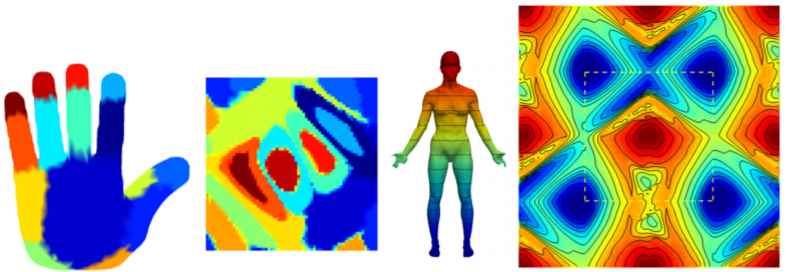
\includegraphics[width=.9\textwidth]{12/19_46}
	\caption{Global parametrization.}\label{fig:param}	
\end{figure}

Everything that a neural network will learn in this domain will be valid in the original domain, since there exists an invertible mapping between the two domains. However you can imagine that such parametrizations are not unique, but there are many ways in which the same surface might be parametrized. Usually these maps introduce \emph{distortion}, in terms of distances, relative angles, local areas not being preserved. Some of these maps will be ``better'' than others, in the sense that will guarantee \emph{invariance} to some transformations, that if you recall is something we seek. Most notably, recall that a \emph{defining property} of convolution is being \emph{translation invariant}, so if we want to define a ``proper'' convolution, we must ensure that this property is satisfied. 

How to define shift invariance on a surface? Recall that surfaces are manifolds, and manifolds are locally Euclidean, so locally to each point of the manifold we can define \emph{vector fields} that encode a translation at all points on the surface, called \emph{translation fields}. This means that at each point we will define a vector space, in which that point will be represented as some vector $\vb{x}$, and there will be a vector-to-vector function $\vb{y} = f(\vb{x})$ that will tell us, for each point in the local neighborhood of that point, what is the effect of the translation, i.e. the position vector $\vb{y}$ to which each point $\vb{x}$ is mapped after the translation.

However, there exists a theorem from differential geometry called the \emph{hairy ball theorem} that states that for a general surface it is not possible to define translation fields that are smooth and also don't have singularities, i.e. points on the surface in which the field is ill-defined. 
\begin{figure}[H]
	\centering
	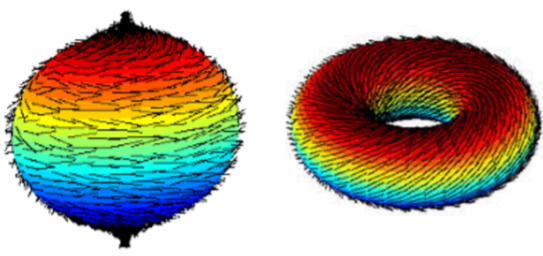
\includegraphics[width=.7\textwidth]{12/20_46_a}
	\caption{Hairy ball theorem. On a sphere we cannot have a translation field without singularities, meaning points in which the translation is not well defined. In this example they are the poles. For other surfaces, like the torus, instead we have no problems.}\label{fig:hairy-ball}	
\end{figure}

This means that we do not have any guarantee of being able to define convolution with this parametric approach, since in general we are not even able to define what translation is, so how can we define an operator that is translation invariant?

In fact, the \emph{torus} is the only surface in which this is possible, since it is the only \emph{closed orientable surface admitting a translational group}.

\begin{figure}[H]
	\centering
	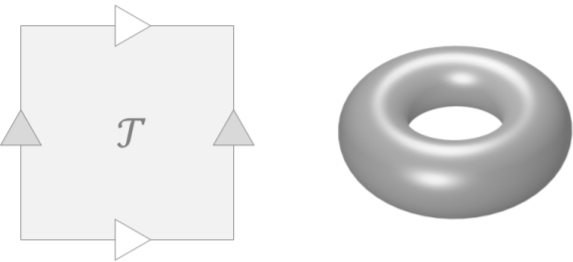
\includegraphics[width=.7\textwidth]{12/20_46_b}
	\caption{Parametrization of a torus.}\label{fig:torus}	
\end{figure}